%% ============================================================
%% 分片 17：原文第 6 节「Loop and Line Operators」（原文 glshort.tex 起于第 4483 行）
%% 由 tools/harvmac2tex.py 从 arXiv 源码（hep-th/0604151v3）自动生成。
%% 只译英文散文；公式、编号、\label、\cite 一律不改。
%% ============================================================

\subsection{紧化到二维}

\label{sec:comptwo}

现在我们要考虑，紧化到二维之后，圈算子或线算子应作何解释。我们取 $M=\Sigma\times C$，其中 $\Sigma$ 与 $C$ 都是黎曼面。设想 $\Sigma$ 远大于 $C$，我们要问：在 $\Sigma$ 上的二维有效理论中，圈算子看起来是什么样子？首先，我们假定 $\Sigma$ 没有边界。

\begin{figure}[htbp]
\centering
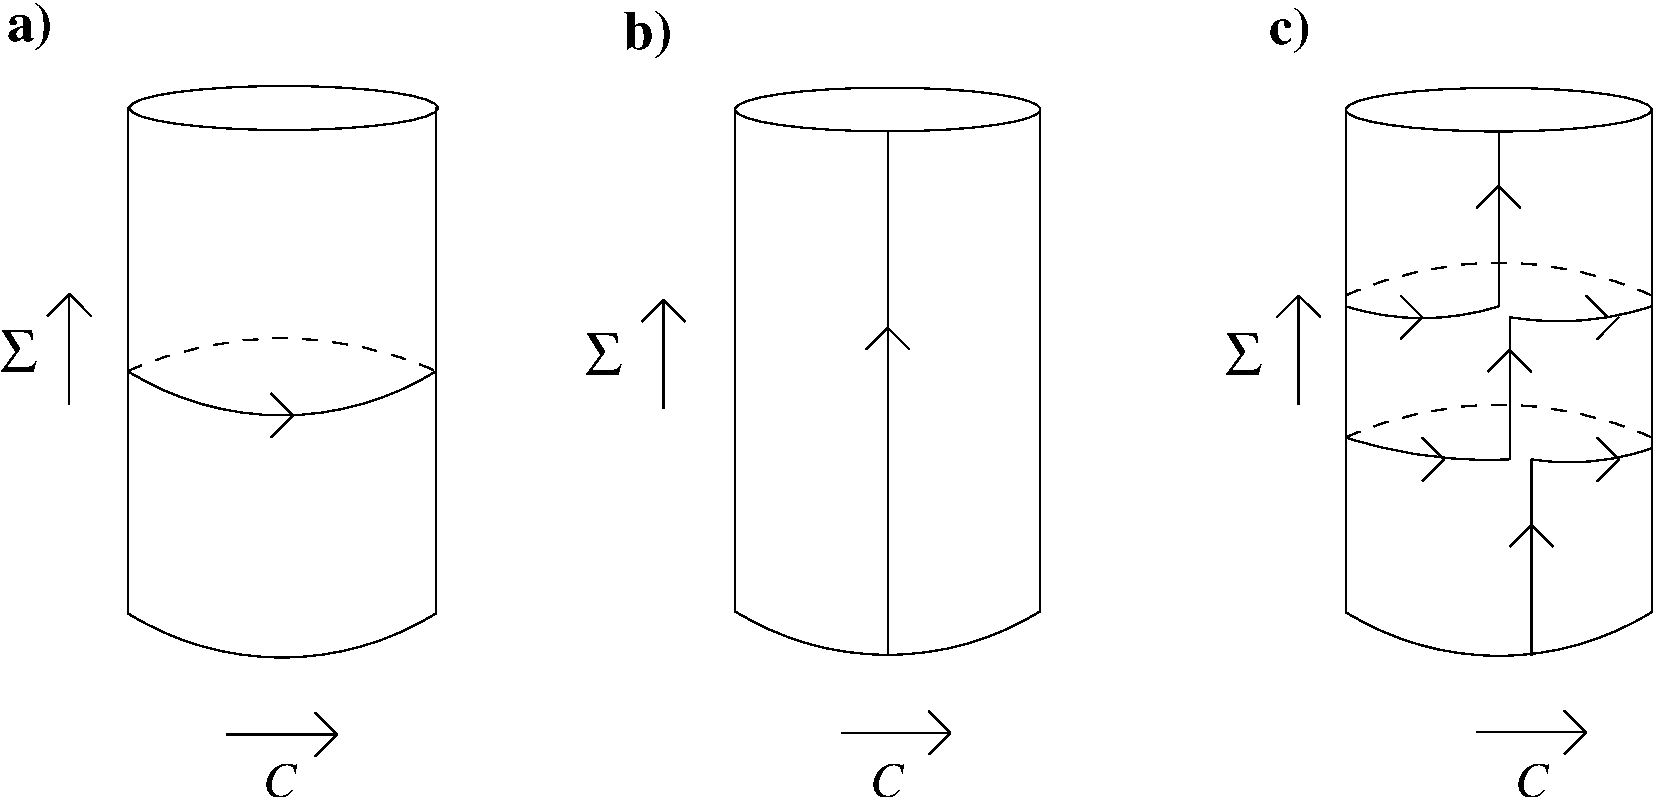
\includegraphics[width=0.75\linewidth]{figures/gla4-1.png}
\caption{四维流形 $\Sigma\times C$ 的示意图，其中 $\Sigma$ 竖直延伸、$C$ 水平延伸。(a) 沿 $C$ 方向传播的 Wilson 线。(b) 沿 $\Sigma$ 方向传播的 Wilson 线。(c) 沿 $\Sigma$ 方向传播、但在两个时刻绕着 $C$ 中一维闭链走一圈的 Wilson 线。（原文 Fig.~4）}
\label{fig:namp-four}  % 原文 \ifig\namp 同名重复（§6 Fig.~4 与 §8 Fig.~11），此处改名以免冲突
\end{figure}
 可以区分出几种情形。一种情形（\namp(a)）是形如 ${{\cal
S}}=p\times {{\cal S}}'$ 的圈，其中 $p$ 是 $\Sigma$ 中的一点，${{\cal S}}'$ 是 $C$ 中的一个圈。显然，支撑在这种圈上的算子，在 $\Sigma$ 上的有效理论中看起来就只是一个点状的局部算子。所有普通的量子场论以及许多 TQFT 都有这样的局部算子，所以在这个例子中，圈算子经过紧化之后变成了 $\Sigma$ 上有效理论中相当普通的东西。

相反的情形（\namp(b)）是 ${{\cal S}}={{\cal S}}''\times q$，其中 ${{\cal S}}''$ 是 $\Sigma$ 中的一个圈，$q$ 是 $C$ 中的一点。此时圈算子在二维有效理论中仍然是圈算子。

一般情形当然是一条在 $\Sigma$ 与 $C$ 中都非平凡地延伸的曲线 ${{\cal S}}$。任何这样的曲线都同伦于一条先在 $\Sigma$ 中延伸、再在 $C$ 中延伸、再在 $\Sigma$ 中延伸……如此反复的曲线，如 \namp(c) 所示。设 $\bar {{\cal S}}$ 是 ${{\cal S}}$ 到 $\Sigma$ 的投影。则 ${{\cal S}}$ 上的圈算子在 $\Sigma$ 上的有效理论中约化为 $\bar {{\cal S}}$ 上的圈算子，并在 $\bar {{\cal S}}$ 的一些特定点上插入了局部算子，这些点正是 ${{\cal S}}$ 绕着 $C$ 延伸的那些点。我们马上会给出这种圈算子的另一种解释。

\begin{figure}[htbp]
\centering
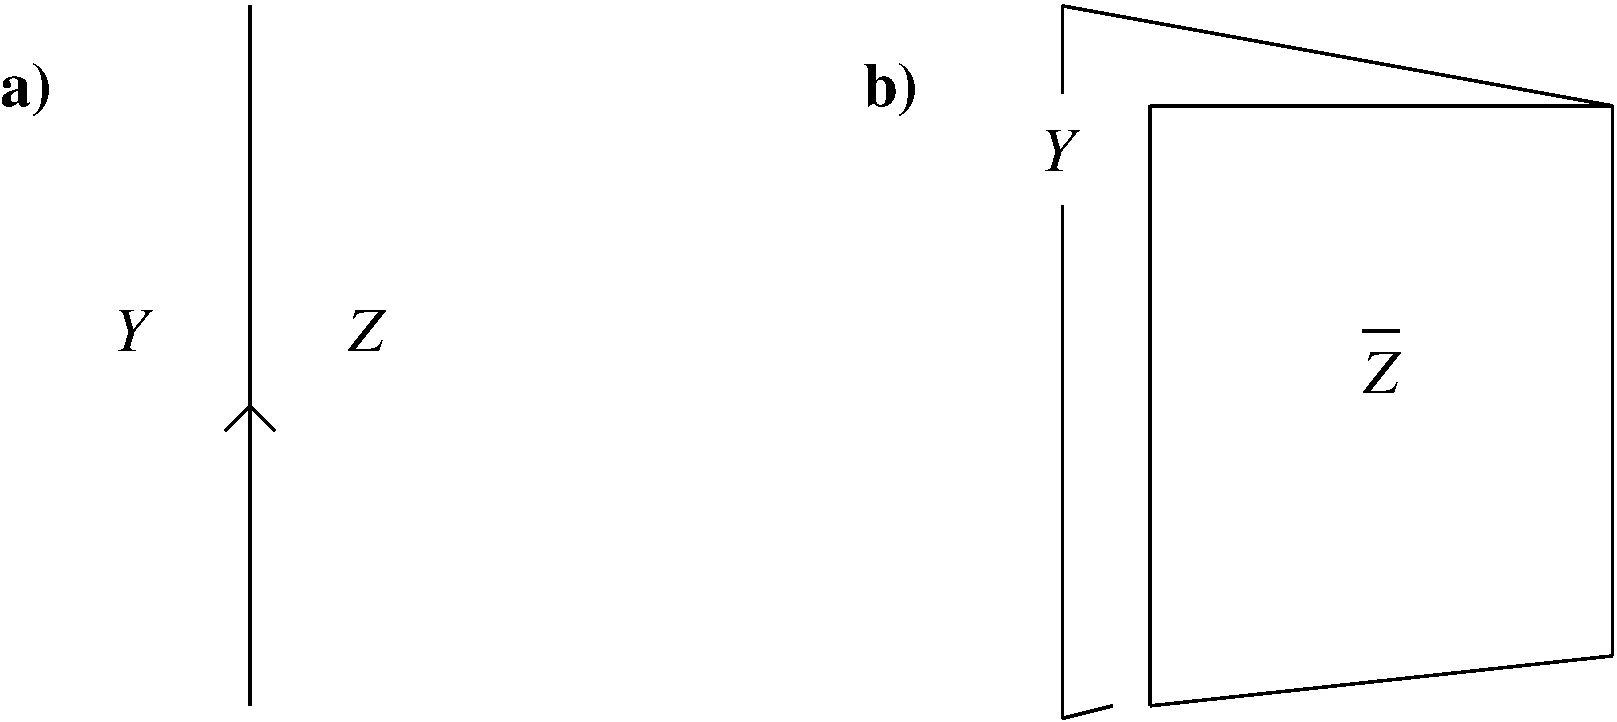
\includegraphics[width=0.75\linewidth]{figures/gla4-2.png}
\caption{(a) 一条线算子把平面分成两个区域，分别由理论 $Y$ 与 $Z$ 标记。(b) 同一图像折叠后的版本，用半平面上的理论 $Y\times \bar Z$ 来解释；其边界由 $(Y,Z)$-膜标记。（原文 Fig.~5）}
\label{fig:tonamp}
\end{figure}
 要点显然在于理解圈算子或线算子在二维中的含义。这里应当注意，一个二维流形局部地被一个一维流形分成两个不相交的区域。因此，一条圈算子或线算子可以产生长程效应；二维有效理论中的耦合常数可能在两侧不同。（Wilson 与 't Hooft 线算子如何能产生这种效应，将在第~\ref{sec:wilbranes}~节中讨论。）这一可能性已包含在 \tonamp(a) 中：那里画出的二维线算子把平面分成两个区域，分别由两个不同的理论 $Y$ 与 $Z$ 标记。

为了把这一情形放进更熟悉的框架，我们可以使用一个「折叠」（folding）技巧（例如见 \cite{ref93,ref94,ref95}）。代价是把区域 $Z$ 的定向反转，得到我们称之为理论 $\bar Z$ 的东西；这样我们就可以把 \tonamp(a)「折叠」，得到一幅类似的图，其中区域 $Y$ 与 $Z$ 位于同一侧，并终止于线算子所在的位置（\tonamp(b)）。

从抽象的观点来看，此时我们得到的是张量积理论 $Y\otimes \bar Z$ 中的一个边界条件。就本文的目的而言，所谓「膜」（brane），一般就是指量子场论中的一个局部边界条件。（换言之，我们的膜全都是 $D$-膜。）我们把乘积理论 $Y\otimes \bar Z$ 中的膜称为 $(Y,Z)$-膜。于是线算子在二维中约化为一个 $(Y,Z)$-膜。

现在我们也能够更好地理解 \namp(c)。此前我们把这一组态解释为带插入局部算子的线算子。折叠之后，二维有效理论被表述在带边界的黎曼面 $\Sigma$ 上，并且在边界上插入了局部算子。它们的存在正是膜物理的特征；一般而言，对任何膜，都存在一个局部算子空间，其元素可以插入到 $\Sigma$ 的由该膜标记的边界分支上。

\begin{figure}[htbp]
\centering
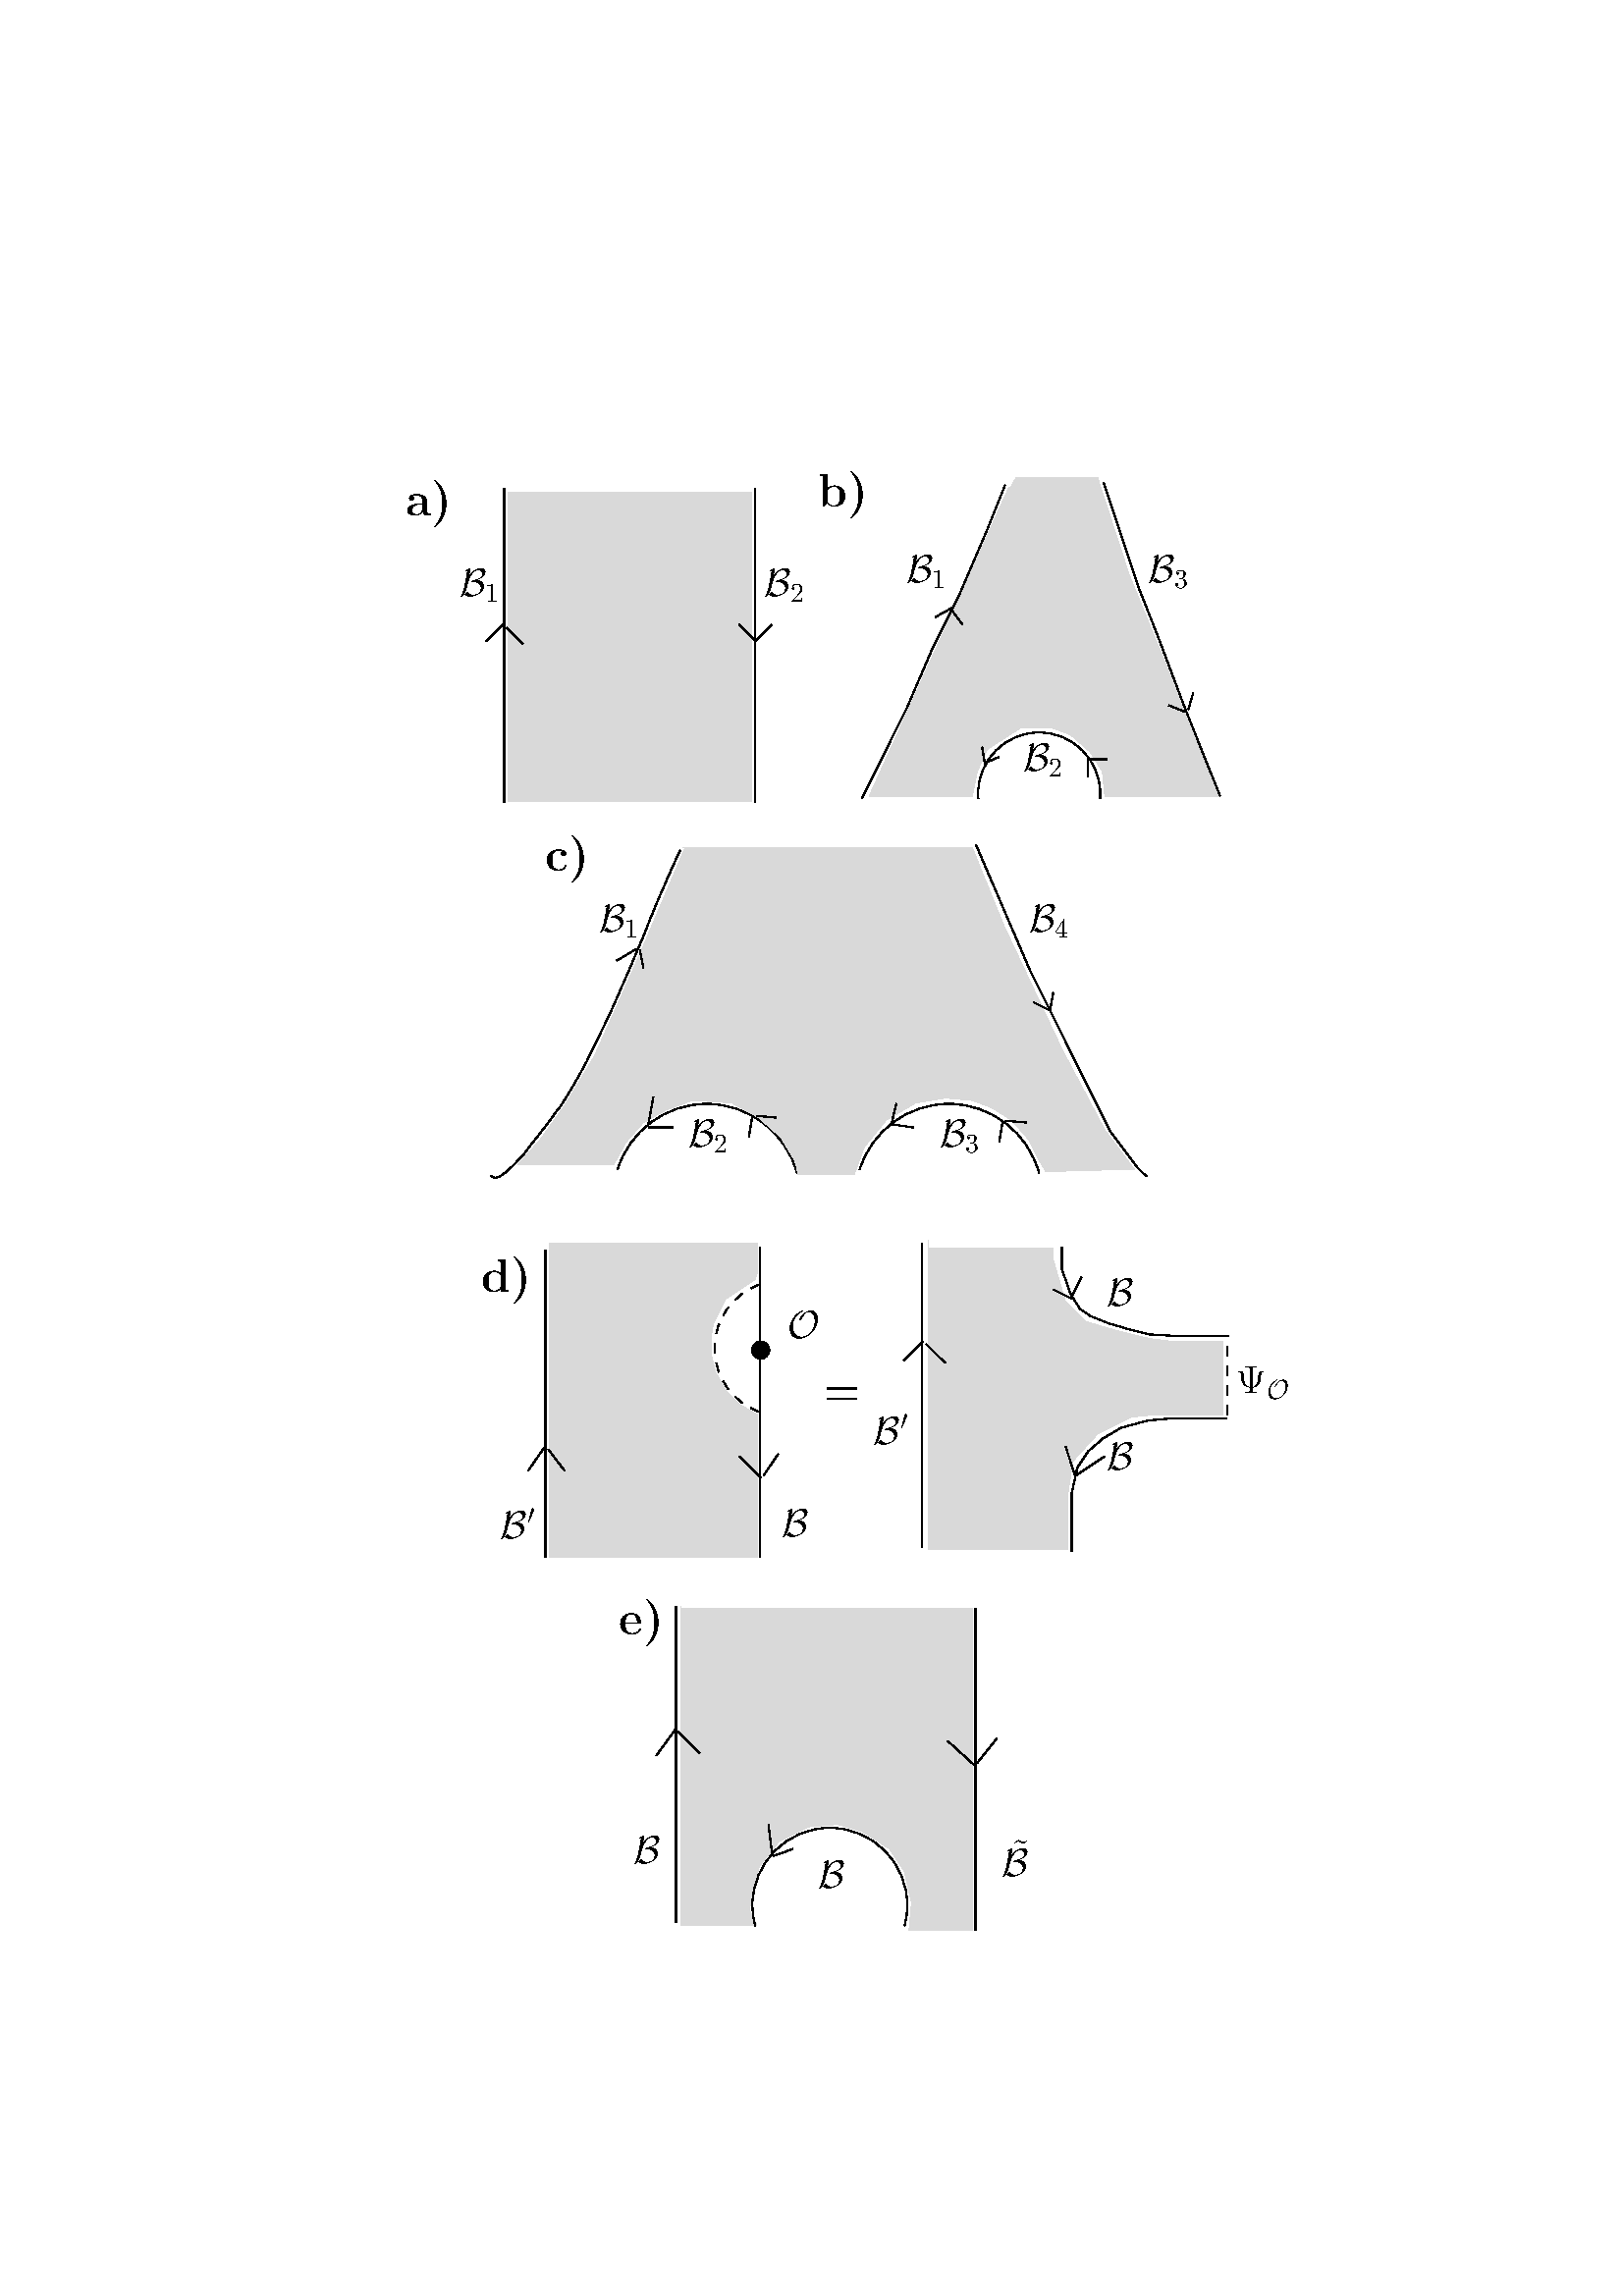
\includegraphics[width=0.75\linewidth]{figures/gla4-3.png}
\caption{(a) $({\cal B}_1,{\cal B}_2)$ 弦的空间。(b) 弦的粘接给出乘积 ${\cal H}_{{\cal B}_1,{\cal B}_2}\otimes {\cal H}_{{\cal B}_2,{\cal B}_3}\to {\cal H}_{{\cal B}_1,{\cal B}_3}$。(c) 由三条弦粘接得到的结合律关系。(d) 可插入由膜 ${\cal B}$ 标记的边界上的局部算子空间 ${\EUO}$ 与空间 ${\cal H}_{{\cal B},{\cal B}}$ 相同。为看出这一点，我们在 ${\EUO}$ 插入点附近的小区域（左图中未着色的区域）作路径积分，得到一个物理态 $\Psi_{\EUO}$，把它插入虚线处即可复现 ${\EUO}$ 的效应；所得图像可写成右图所示的形式。(e) 对每个 ${\cal B}$ 与 $\tilde{\cal B}$，空间 ${\cal H}_{{\cal B},\tilde{\cal B}}$ 是代数 ${\cal H}_{{\cal B},{\cal B}}$ 的一个模。（原文 Fig.~6）}
\label{fig:dunamp}
\end{figure}

 让我们回忆如何刻画这样的局部算子。这也有助于回忆关于膜的几个基本事实。对每个二维量子场论 $X$ 以及每一对膜 ${\cal B}_1$ 与 ${\cal B}_2$，都可以定义一个向量空间 ${\cal H}_{{\cal
B}_1,{\cal B}_2}$，即 $({\cal B}_1,{\cal B}_2)$ 弦的空间。在酉量子场论中，这些空间是 Hilbert 空间；即便没有酉性，${\cal H}_{{\cal B}_1,{\cal B}_2}$ 也对偶于 ${\cal H}_{{\cal B}_2,{\cal B}_1}$。${\cal H}_{{\cal
B}_1,{\cal B}_2}$ 的定义方式是：在 $\Sigma=\Bbb{R}\times I$ 上量子化理论 $X$，其中 $I$ 是单位区间，其两端分别由 ${\cal B}_1$ 与 ${\cal B}_2$ 标记（\dunamp(a)）。${\cal H}_{{\cal B}_1,{\cal B}_2}$ 也称为该理论在 $I$ 两端给定边界条件下的物理态空间。

而在拓扑场论中，对任意膜 ${\cal
B}_1,{\cal B}_2,$ 与 $ {\cal B}_3$，都有自然映射 ${\cal H}_{{\cal
B}_1,{\cal B}_2}\otimes {\cal H}_{{\cal B}_2,{\cal B}_3}\to {\cal
H}_{{\cal B}_1,{\cal B}_3}$，它们由把黎曼面粘接起来定义（\dunamp(b)）。（在没有拓扑不变性的二维量子场论中，必须把度规或曲面的共形结构考虑进去，其结果是一个类似的讨论会导出算子乘积展开。）这些映射满足显然的结合律关系，即当三条弦粘接时（\dunamp(c)），不必说清哪两条先粘接。特别地，把所有膜 ${\cal B}_i$ 都取为 ${\cal B}$，我们发现 ${\cal H}_{{\cal B},{\cal B}}$ 总具有结合代数的自然结构。

事实上，在 TQFT 中，可插入由膜 ${\cal B}$ 标记的边界上的局部算子空间 ${\EUO}$ 与 ${\cal H}_{{\cal B},{\cal B}}$ 相同，因为（\dunamp(d)）在这样的 ${\EUO}$ 附近施加一次「切割」操作，就会显示出 ${\cal H}_{{\cal B},{\cal B}}$ 的一个元素。由类似的推理（\dunamp(e)），我们发现，对任意 ${\cal B}$ 与 $ \tilde{\cal
B}$，${\cal H}_{{\cal B}, \tilde{\cal B}}$ 总具有左 ${\cal H}_{{\cal B},{\cal B}}$-模的自然结构。同样，它具有右 ${\cal H}_{\tilde
{\cal B},\tilde{\cal B}}$ 模的自然结构。事实上，${\cal H}_{{\cal B},
\tilde{\cal B}}$ 是一个 $({\cal H}_{{\cal B},{\cal B}},{\cal
H}_{\tilde{\cal B},\tilde{\cal B}})$ 双模。这只不过是说，可以用 ${\cal H}_{{\cal B},{\cal B}}$ 在左边贴一条弦来作用，也可以用 ${\cal H}_{\tilde{\cal B},\tilde{\cal
B}}$ 在右边贴一条弦来作用，而且这两个作用交换。

\begin{yizhu}[易错点]
圈算子约化到 $\Sigma$ 上并不总是圈算子。按其在 $C$ 与 $\Sigma$ 中走向的不同要分三类：（a）$p\times{{\cal S}}'$ 约化为 $\Sigma$ 上的点状局部算子；（b）${{\cal S}}''\times q$ 仍是 $\Sigma$ 上的圈算子；（c）一般曲线约化为 $\bar{{\cal S}}$ 上的圈算子加若干特定点处的局部算子插入。把（a）也当成「圈算子」留在二维理论里是最常见的误读。
\end{yizhu}

\begin{yizhu}[物理图像]
折叠技巧（folding trick）的要点：线算子把平面分成标记为 $Y$ 与 $Z$ 的两个区域；把 $Z$ 反定向、改称 $\bar Z$ 并把图折过来，就得到 $Y\otimes\bar Z$ 张量积理论中位于半平面上的一个边界条件，即 $(Y,Z)$-膜。于是「线算子」被翻译成「膜（=局部边界条件）」。这一步也是后文把四维线算子变成二维膜、进而用膜范畴讨论线算子的起点。
\end{yizhu}

\begin{yizhu}[易错点]
${\cal H}_{{\cal B}_1,{\cal B}_2}$ 是量子化所得的态空间，不是某个几何上预先给定的向量空间：它由在 $\Sigma=\Bbb{R}\times I$ 上量子化、两端分别贴膜 ${\cal B}_1$ 与 ${\cal B}_2$ 定义，并要求 $I$ 是单位区间。粘接黎曼面给出乘积 ${\cal H}_{{\cal B}_1,{\cal B}_2}\otimes{\cal H}_{{\cal B}_2,{\cal B}_3}\to{\cal H}_{{\cal B}_1,{\cal B}_3}$，其结合律使 ${\cal H}_{{\cal B},{\cal B}}$ 成为结合代数；对一般的 ${\cal B},\tilde{\cal B}$，${\cal H}_{{\cal B},\tilde{\cal B}}$ 是左 ${\cal H}_{{\cal B},{\cal B}}$-模、右 ${\cal H}_{\tilde{\cal B},\tilde{\cal B}}$-模，即双模，两种作用交换。
\end{yizhu}

\begin{yizhu}[含糊点拨]
原文特意声明「by a brane, in general, we simply mean a local boundary condition in a quantum field theory」并补一句「our branes are all $D$-branes」。按 GLOSSARY 的定译，本文一律译作「膜」而不加 D-；但读者应记住这里的膜就是局部边界条件（特殊的 D-膜），并非任意延展对象。
\end{yizhu}

\begin{yizhu}[物理图像]
图 6(d) 的「切割」论证是 TQFT 中「局部算子 = 边界态」的标准等价：在算子 ${\EUO}$ 的插入点周围的小区域里作路径积分，得到边界上的一个物理态 $\Psi_{\EUO}$，把这个态插回虚线处就复现了 ${\EUO}$ 的效应。正因如此，${\EUO}$ 的空间才等于 ${\cal H}_{{\cal B},{\cal B}}$；而在非拓扑的二维量子场论中，对应的构造会给出算子乘积展开。
\end{yizhu}

\begin{yizhu}[原文疑误]
原文第 136 行作 「can be inserted on a a boundary labeled by ...」，其中「a a」是重复冠词，系底本笔误（应为单个 a）。译文按单数不定冠词处理，语义不受影响。
\end{yizhu}
